\chapter{Problem}
\label{cha:problem}

\sloppy

\section{Motivation}
\label{sec:motivation}

Text has evolved with the advance of technology resulting in the creation of \textit{markup languages} \cite{markuplanguages}. Markup languages work by adding annotations to text, the annotations being also known as tags, that allow to add additional information to the text. Each markup language has its own tags and each of those tags add a different meaning to the text encapsulated within them. In order to use markup languages the users can write the text and add all the tags manually, either by fully writing them or by using some kind of text helpers such as text editors with IntelliSense\footnote{\href{https://www.techopedia.com/definition/24580/intellisense}{Intellisense Definition}} which can help diminish the errors caused by manually writing the tags. But even with text helpers the resulting document can violate the restrictions of the respective markup language because the editors don't actually enforce the language rules. 

\noindent
The most common markup language is the \ac{HTML} language, which is heavily used in Web applications. Other uses of the \ac{HTML} language are writing emails, writing reports, etc. The function of \ac{HTML} in Web applications is to define the user-interface, which is also known as the view of the website. To generate the end view the most common solution is the usage of \textit{template engine}  solutions, which can be considered the \textit{controller} which is responsible for joining the domain data with the views. This approach separates the \textit{view} from the \textit{controller}, which allows both of the different layers of a project to be more independent. But, with the usage of \textit{template engines}, there is another layers of complexity between the \textit{view} and the \textit{controller}, since both of these aspects of the project use different programming languages. 

\noindent
In the following examples we will show the Java code necessary to join a template, the \texttt{view}, that generates a table in \ac{HTML} with a list of  \texttt{TableElement} objects, Listing \ref{lst:companyinfo}, which is the \texttt{domain data} which describes information about a company, its country and a name of a contact inside the company. We will present different examples in order to show how the complexity of the actions we want to perform affect the different solutions (the template engines and the \texttt{xmlet} solution).

\bigskip

\lstset{language=java, morekeywords={TableElement, String}}

\begin{minipage}{\linewidth}
\begin{lstlisting}[caption={Company Information Table Element}, label={lst:companyinfo}]
class TableElement{
    String company;
    String contact;
    String country;

    TableElement(String company, String contact, String country){
        this.company = company;
        this.contact = contact;
        this.country = country;
    }
}
\end{lstlisting}
\end{minipage} 

\noindent
The resulting table should be similar to the one presented in Figure \ref{img:tableelement}, which is the example used in the Table HTML element page\footnote{\href{https://www.w3schools.com/html/html_tables.asp}{Table Element at W3C}} of \ac{W3C}. 

\bigskip

\begin{figure}[H]
	\centering
	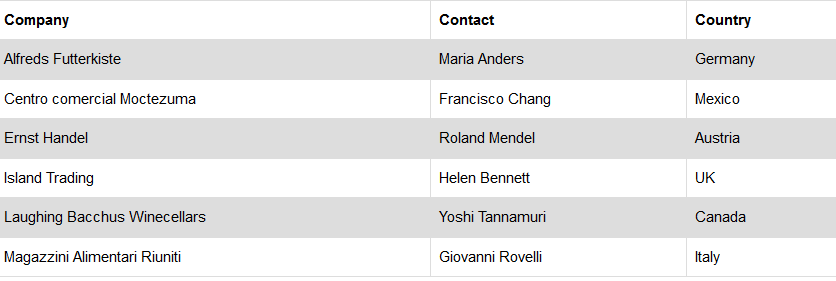
\includegraphics[width=1\textwidth]{tablew3c}
	\caption{Table Element Page at W3C}
	\label{img:tableelement}
\end{figure}

\noindent
To represent that table using the Mustache idiom we have the following template, Listing \ref{lst:mustacheex1template}.

\bigskip

\lstset{language=html, morekeywords={tableElements}}

\begin{minipage}{\linewidth}
\begin{lstlisting}[caption={Company Information Table Element}, label={lst:mustacheex1template}]
<table>
    <tr>
        <th>company</th>
        <th>contact</th>
        <th>country</th>
    </tr>
    {{#tableElements}}
    <tr>
        <td>{{company}}</td>
        <td>{{contact}}</td>
        <td>{{country}}</td>
    </tr>
    {{/tableElements}}
</table>
\end{lstlisting}
\end{minipage} 

\noindent
In this situation it is possible to define the header rows directly in the template, adding the data rows of the table dynamically by receiving an \texttt{Iterable<TableElement>} named \texttt{tableElements} as shown in Listing \ref{lst:mustacheex1code}. Since the names of the fields are known they can be directly referenced in the \texttt{td} elements.

\bigskip

\lstset{language=java, morekeywords={Writer, MustacheFactory, OutputStreamWriter, DefaultMustacheFactory, System, Mustache, compile, StringReader, execute, Iterable, getTableElements, TableElement, flush}}

\begin{minipage}{\linewidth}
\begin{lstlisting}[caption={Mustache With Iterable<TableElement>}, label={lst:mustacheex1code}]
Writer writer = new OutputStreamWriter(System.out);
MustacheFactory mf = new DefaultMustacheFactory();

// String template = Previous Listing

Mustache mustache = mf.compile(new StringReader(template), "");

mustache.execute(writer, new Object(){
    Iterable<TableElement> tableElements = getTableElements();
});

writer.flush();
\end{lstlisting}
\end{minipage} 

\newpage

\noindent
Moving this example to the desired implementation of the \texttt{xmlet} solution we would have the following code present in Listing \ref{lst:htmlapiex1}.

\lstset{language=java, morekeywords={TableElement, CustomVisitor, List, getTableElements, Element, Table, tr, th, text, binder, forEach, td, accept, System, out, println, getResult}}

\begin{minipage}{\linewidth}
\begin{lstlisting}[caption={Mustache With Iterable<TableElement>}, label={lst:htmlapiex1}, literate={º}{\textdegree}1]
CustomVisitor<List<TableElement>> visitor = 
    new CustomVisitor<>(getTableElements());
Table<Element> table = new Table<>();

table.tr()
        .th().text("company").º()
        .th().text("contact").º()
        .th().text("country").º().º()
     .<List<TableElement>>binder((tableObj, tableElements) ->
        tableElements.forEach(tableElement ->
            tableObj.tr()
                        .td().text(tableElement.company).º()
                        .td().text(tableElement.contact).º()
                        .td().text(tableElement.country)
        )
     );

table.accept(visitor);
System.out.println(visitor.getResult());
\end{lstlisting}
\end{minipage} 

\noindent
The complexity between the two previously presented seems similar, since the example is straightforward. But what if we wanted to create a template that instead of using an \texttt{Iterable<TableElement>} as the \texttt{domain data} used an \texttt{Iterable<T>}? This new solution would imply that the programmer doesn't have knowledge about the fields of the type to present on the table and therefore won't be able to use the same templates. To solve this new problem both solutions have to use reflection in order to obtain information about the concrete type represented by the \texttt{T} type. Since the \texttt{xmlet} solution is integrated in the Java environment it's easier to solve this issue. The solution uses reflection to obtain the field information of the type \texttt{T} and then uses the field information to generate the static part of the template represented by the header of the table and then it binds the \texttt{table} element to a function that receives the table data, a \texttt{List<T>} variable,  and creates  the table row elements, \texttt{tr}, accordingly. The final table is generated when the \texttt{table} element invokes the method \texttt{accept} receiving a concrete visitor implementation, i.e. variable \texttt{visitor}, which contains the concrete table data, i.e. variable \texttt{elementList}.

\lstset{language=java, morekeywords={List, T, getTableElementsAsT, Field, isEmpty, ArrayList, asList, get, getClass, getDeclaredFields, CustomVisitor, Table, Arrays, Element, Tr, forEach, tr, th, text, getName, binder, td, toString, IllegalAccessException, printStackTrace, accept, getResult, System, out, println}}

\begin{minipage}{\linewidth}
\begin{lstlisting}[caption={Mustache With Iterable<TableElement>}, label={lst:htmlapiex2}, literate={º}{\textdegree}1]
List<T> elementList = getTableElementsAsT();
List<Field> fields = 
   elementList.isEmpty() ? 
      new ArrayList<>() : 
      Arrays.asList(elementList.get(0).getClass().getDeclaredFields());

CustomVisitor<List<T>> visitor = new CustomVisitor<>(elementList);
Table<Element> table = new Table<>();
Tr<Table<Element>> titleRow = table.tr();

fields.forEach(field -> titleRow.th().text(field.getName()));

table.<List<T>>binder((tableObj, tableElements) ->
        tableElements.forEach(tableElement -> {
           Tr<Table<Element>> tableRow = tableObj.tr();
           fields.forEach(field -> {
             try {
                tableRow.td().text(field.get(tableElement).toString());
             } catch (IllegalAccessException e) {
                e.printStackTrace();
             }
           });
     }));

table.accept(visitor);
System.out.println(visitor.getResult());
\end{lstlisting}
\end{minipage} 

\noindent
The Mustache solution to this new problem is a bit more complex, compared to the first example which used a \texttt{Iterable<TableElement>} as the \texttt{domain data}. The new template, Listing \ref{lst:mustacheex2template}, is fairly similar, it now receives the \texttt{headerNames} variable which contains the names of the field of the given \texttt{T} type which should be inserted in the table headers and also receives the \texttt{data} variable. This \texttt{data} variable is a work around to the weaknesses of the syntax provided by the Mustache idiom, it's a \texttt{List<List<String>>} object, with the inner list being the a list containing the values present in the fields of a single instance of type \texttt{T} and the outer list being the list that mimics a list of \texttt{T}. This solution was forced onto the programmer since Mustache doesn't provide enough tools to do this in other way. The first approach to this problem was to use a \texttt{Map<T, List<String>>} which associated a \texttt{T} object with a list of \texttt{String} representing the names of the fields of \texttt{T}. This didn't work since Mustache doesn't allow multiple contexts which was needed in order to access the object and then access the list to write the placeholders for the class fields, such as the \texttt{td} elements in Listing \ref{lst:mustacheex1template}.

\lstset{language=html, morekeywords={headerNames, data}}

\begin{minipage}{\linewidth}
\begin{lstlisting}[caption={Company Information Table Element}, label={lst:mustacheex2template}]
<table>
    <tr>
    {{#headerNames}}
        <th>{{.}}</th>
    {{/headerNames}}
    </tr>
    {{#data}}
    <tr>
       {{#.}}
       <td>{{.}}</td>
       {{/.}}
    </tr>
    {{/data}}
</table>
\end{lstlisting}
\end{minipage} 

\noindent
This approach to the problem generated code that is more complex in the Java language. The code present in Listing \ref{lst:mustacheex2code} is the Java code needed to prepare the \texttt{Object} that has the context for the template, containing the \texttt{headerNames} and \texttt{data} variables.

\lstset{language=java, morekeywords={Writer, OutputStreamWriter, System.out, MustacheFactory, DefaultMustacheFactory, Mustache, compile, StringReader, execute, Object, List, getNames, getData, getFields, stream, map, getName, collect, Collectors, toList, Field, ArrayList, getTableElementsAsT, forEach, add, get, toString, IllegalAccessException, printStackTrace, collect, Collectors, toList, findFirst, ifPresent, addAll, Arrays, asList, getClass, getDeclaredFields, flush, String}}

\begin{minipage}{\linewidth}
\begin{lstlisting}[caption={Mustache With Iterable<TableElement>}, label={lst:mustacheex2code}]
Writer writer = new OutputStreamWriter(System.out);
MustacheFactory mf = new DefaultMustacheFactory();
Mustache mustache = mf.compile(new StringReader(template), "");

mustache.execute(writer, new Object(){
    List<String> headerNames = getNames();
    List<List<String>> data = getData();

    List<String> getNames() {
        return getFields().stream().map(Field::getName)
                          .collect(Collectors.toList());
    }

    List<List<String>> getData() {
        List<Field> fields = getFields();

        return getTableElementsAsT()
                .stream()
                .map(elem ->
                    fields.stream()
                          .map(field -> {
                              try {
                                  return field.get(elem).toString();
                              } catch (IllegalAccessException e) {
                                  e.printStackTrace();
                              }
                              return "";
                         }).collect(Collectors.toList()))
                .collect(Collectors.toList());
    }

    private List<Field> getFields() {
        List<Field> fields = new ArrayList<>();

        getTableElementsAsT()
           .stream().findFirst().ifPresent(elem -> 
              fields.addAll(
                  Arrays.asList(elem.getClass().getDeclaredFields())));
        return fields;
    }
});
writer.flush();
\end{lstlisting}
\end{minipage} 

\noindent
With this comparison we observe that for simple problems both the template engines and the \texttt{xmlet} solution are viable but when the problems increase in complexity the template engine solutions start to present their weaknesses while the \texttt{xmlet} solution keeps the same complexity in its solution. We can also observe that when complexity escalates the extra coded needed to compensate the weaknesses of the template engines degrade the overall performance of the application.

\section{Problem Statement}
\label{sec:problemstatement}

The problem that's being presented revolves around the handicaps of template engines, the lack of compilation of the language used within the template, the performance overhead that it introduces and the issues that it was when the complexity increases, as it was presented in the previous Section \ref{subsec:templateengineshandicaps}. To tackle those handicaps we suggested the automated generation of a strongly typed fluent interface. In order to show how that \ac{API} will effectively work we will now present a small example which consists on the \texttt{html} element, Listing \ref{lst:codegenerationexample}, described in \ac{XSD} of the \ac{HTML}5 language definition. The presented example is simplified for explanation purposes.

\bigskip

\lstset{
	language=XML,
	morekeywords={xs:element, name, xs:complexType, xs:choice, ref, xs:attributeGroup, xs:attribute, type}
}

\begin{minipage}{\linewidth}
\begin{lstlisting}[caption={Code Generation XSD Example},captionpos=b, ,label={lst:codegenerationexample}]
<xs:attributeGroup name="commonAttributeGroup">
    <xs:attribute name="someAttribute" type="xs:string">
</xs:attributeGroup>

<xs:element name="html">
    <xs:complexType>
        <xs:choice>
            <xs:element ref="body"/>
            <xs:element ref="head"/>
        </xs:choice>
        <xs:attributeGroup ref="commonAttributeGroup" />
        <xs:attribute name="manifest" type="xs:string" />
    </xs:complexType>
</xs:element>
\end{lstlisting}
\end{minipage}

\noindent
With this example there is a multitude of classes that need to be created, apart from the always present supporting infrastructure that will be presented in Section \ref{sec:supportinginfrastructure}. 

\begin{itemize}
	\item Html Element - A class that represents the \texttt{Html} element (Listing \ref{lst:htmlclass}), deriving from \texttt{AbstractElement}.
	\item Body and Head Methods - Both methods present in the \texttt{Html} class (Listing \ref{lst:htmlclass}) that add \texttt{Body} (Listing \ref{lst:bodyclass}) and \texttt{Head} (Listing \ref{lst:headclass}) instances to \texttt{Html} children list.
	\item Manifest Method - A method present in \texttt{Html} class (Listing \ref{lst:htmlclass}) that adds an instance of the \texttt{Manifest} attribute (Listing \ref{lst:manifestattributeclass}) to the \texttt{Html} attribute list.
\end{itemize}

\lstset{language=Java, morekeywords={AbstractElement, CommonAttributeGroup, Body, addChild, Head, String, AttrManifest, addAttr}}

\begin{lstlisting}[caption={Html Element Class},captionpos=b,label={lst:htmlclass}]
class Html extends AbstractElement implements CommonAttributeGroup {
    public Html() { }
    
    public void accept(Visitor visitor){
		visitor.visit(this);    
    }
    
    public Html attrManifest(String attrManifest) {
        return this.addAttr(new AttrManifest(attrManifest));
    }
    
    public Body body() { return this.addChild(new Body()); }
        
    public Head head() { return this.addChild(new Head()); }
}
\end{lstlisting}

\begin{itemize}
	\item Body and Head classes - Classes for both \texttt{Body} (Listing \ref{lst:bodyclass}) and \texttt{Head} (Listing \ref{lst:headclass}) elements, similar to the generated \texttt{Html} class (Listing \ref{lst:htmlclass}). The class contents will be dependent on the contents present in the concrete \texttt{xsd:element} nodes.
\end{itemize}

\bigskip

\begin{minipage}{\linewidth}
\begin{lstlisting}[caption={Body Element Class},captionpos=b,label={lst:bodyclass}]
public class Body extends AbstractElement {
    //Similar to Html, based on the contents of the respective
    //xsd:element node.
}
\end{lstlisting}
\end{minipage}

\bigskip

\begin{minipage}{\linewidth}
\begin{lstlisting}[caption={Head Element Class},captionpos=b,label={lst:headclass}]
public class Head extends AbstractElement {
    //Similar to Html, based on the contents of the respective 
    //xsd:element node.
}
\end{lstlisting}
\end{minipage}

\begin{itemize}
	\item Manifest Attribute - A class that represents the \texttt{Manifest} attribute  (Listing \ref{lst:manifestattributeclass}), deriving from \texttt{BaseAttribute}.
\end{itemize}

\bigskip

\lstset{language=Java, morekeywords={String, BaseAttribute}}

\begin{minipage}{\linewidth}
\begin{lstlisting}[caption={Manifest Attribute Class},captionpos=b,label={lst:manifestattributeclass}]
public class AttrManifestString extends BaseAttribute<String> {
    public AttrManifestString(String attrValue) {
        super(attrValue);
    }
}
\end{lstlisting}
\end{minipage}

\begin{itemize}
	\item CommonAttributeGroup Interface - An interface with default methods that add the group attributes to the concrete element (Listing \ref{lst:commonattributegroup}).
\end{itemize}

\bigskip

\lstset{language=Java, morekeywords={addAttr, Html, Element, String, SomeAttribute}}

\begin{minipage}{\linewidth}
\begin{lstlisting}[caption={CommonAttributeGroup Interface},captionpos=b,label={lst:commonattributegroup}]
public interface CommonAttributeGroup extends Element {
    default Html attrSomeAttribute(String attributeValue) {
        this.addAttr(new SomeAttribute(attributeValue));
        return this;
    }
}
\end{lstlisting}
\end{minipage}

\noindent
By analyzing this little example we can observe how the \texttt{xmlet} solution implements one of its most important features that was lacking in the template engine solutions, the user is only allowed to generate a tree of elements that follows the rules specified in the \ac{XSD} file of the given language, e.g. the user can only add \texttt{Head} and \texttt{Body} elements as children to the \texttt{Html} element and the same goes for attributes as well, the user can only add a \texttt{Manifest} or \texttt{SomeAttribute} objects as attribute. This solution effectively uses the Java compiler to enforce the specific language restrictions, most of them at compile time. The other handicaps are also solved, the template can now be defined within the Java language eradicating the necessity of textual files that still need to be loaded into memory and resolved by the template engine. The complexity and flexibility issues are also tackled by moving all the parts of the problem to the Java language, it removes the necessity of additional syntax and now the Java syntax can be used to create the templates.

\section{Approach}
\label{sec:approach}

The approach to achieve a solution was to divide the problem into three distinct aspects, as previously stated in the \ref{sec:thesisstatement}. 

\noindent
The XsdParser project will be an utility project which is needed in order to parse all the external \ac{DSL} rules present in the \ac{XSD} document into structured Java classes. 

\noindent
The XsdAsm is the most important aspect of the \texttt{xmlet} solution, since it is the aspect which will deal with the generation of all the bytecodes that make up the classes of the Java fluent interface. This project should translate as many rules of the parsed language definition, its \ac{XSD} file, into the Java language in order to make the resulting \ac{API} as much similar as possible to the language definition.

\noindent
The HtmlApi will be a representation of client aspect of \texttt{xmlet} solution. It's a concrete client of the XsdAsm project, it will use the \ac{HTML}5 language definition file in order to request of XsdAsm a strongly typed fluent interface, named HtmlApi. This use case is meant to be used by the HtmlFlow \ac{API}, which will implement its own Visitor in order to use the HtmlApi to write well formed \ac{HTML} documents. At the moment HtmlFlow already supports a set of the \ac{HTML} elements which were created manually and the rest of the library interacts with those elements in order to write the \ac{HTML} files. By using the HtmlApi the HtmlFlow will support the whole \ac{HTML} syntax. 